\documentclass[18pt]{beamer}
\usepackage{templates/beamerthemekit}
\usepackage[export]{adjustbox}
% \usepackage{templates/beamerthemekitwide}

%\titlelogo{mylogo}
% \usepackage{templates/tikzkit}
% \usepackage{templates/tikzuml}
%\titleimage{myimage}
\titlelogo{myimage}


\title[Short title]{Erstellung und Evaluierung stochastischer Regressionsmodelle auf Basis heterogener Messnetzwerke.}
\subtitle{Bachelor Arbeit, Vortrag}
\author{Stanislav Arnaudov}

\institute{TECO - Das Telecooperation Office}
\usepackage[citestyle=authoryear,bibstyle=numeric,hyperref,backend=biber]{biblatex}
\addbibresource{templates/example.bib}
\bibhang1em
 
\begin{document} 

% \selectlanguage{english}
\selectlanguage{ngerman}


\begin{frame}
 \titlepage
\end{frame}

\begin{frame}
  \frametitle{Motivation}
  
  \begin{columns}
    \begin{column}{0.4\textwidth}
      Betrachtete Probleme:
      \begin{itemize}
      \item Verbesserung die Vorhersagemöglichkeiten von Modellen durch Hinzunahme unsicherer Sensoren.
      \item Die Qualität von den verwendeten Sensoren bestimmen.
      \item Die Genauigkeit bei Messen durch Berücksichtigung der Unsicherheit erhöhen.
      \end{itemize}
      
    \end{column}
    \begin{column}{0.6\textwidth}
      \begin{center}
        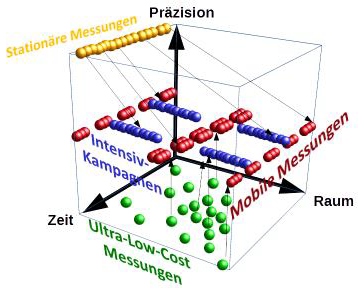
\includegraphics[scale=0.5]{images/motivation}
      \end{center}
    \end{column}
  \end{columns}
  
\end{frame}

\begin{frame}
  \frametitle{Betrachtete Daten}
  Untersucht wird ein heterogenes Netzwerk von Sensoren, die den Feinstaub in Stuttgart herum messen.\\
  Daten aus:
  \begin{itemize}
  \item LU-BW (Landesanstalt für Umwelt, Messungen und Naturschutz Baden-Württemberg) - \textbf{3 Sensoren} hocher Qualität. Man kann diese als Ground-Truth annehmen.
  \item luftdate.info - Daten von einer großen Menge unsicherer Sensoren von niedriger Qualität.
  \end{itemize}
  Zeitraum: 2017.
  
\end{frame}

\begin{frame}
  \frametitle{Stochastische Regressionsmodelle}
  Stochastische Regressionsmodelle:
  \begin{itemize}
  \item Bayesian Neural Networks
    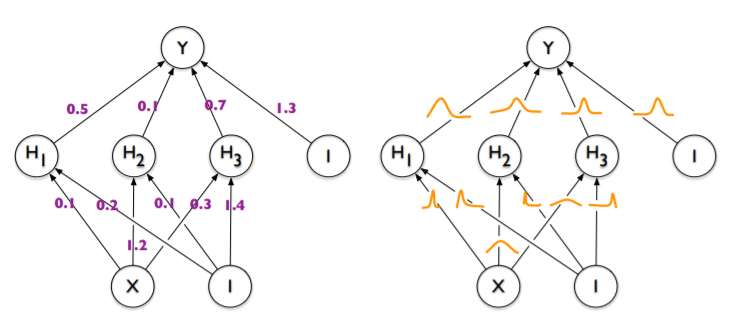
\includegraphics[scale=0.35]{images/bnn}
  \item Mixtures of Gaussian Process Experts
  \end{itemize}
\end{frame}

\begin{frame}[]
  \frametitle{Training}
  \begin{itemize}
    \item Training mit Zeitreihen von allen Sensoren.
  \item Loss Function - Wahrscheinlichkeitsverteilung (Proper Scoring Rules).
  \end{itemize}
  
\end{frame}

\begin{frame}
  \frametitle{Evaluierung von den aufgebauten Modellen}
  Eigenschaften von den untersuchten Modellen
  \begin{itemize}
  \item Wahrscheinlichkeitsverteilung und nicht Punktschätzung
    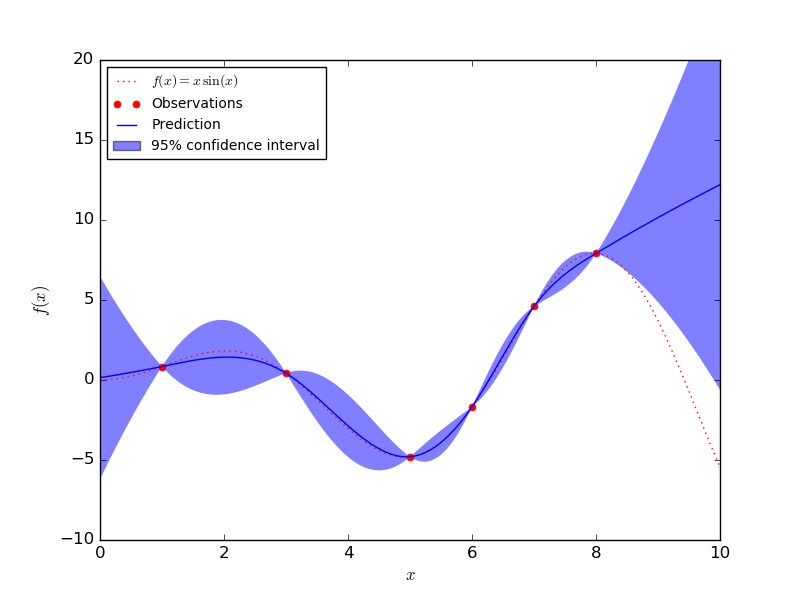
\includegraphics[scale=0.2]{images/graph_1}
    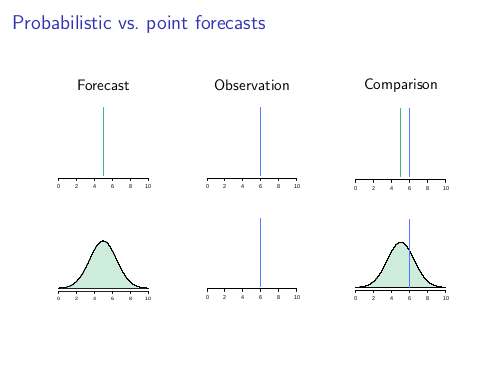
\includegraphics[scale=0.4]{images/graph_2}
  \end{itemize}
  Proper Scoring Rules - Evaluierung von den vorhergesagten Verteilungen.
\end{frame}

\end{document}
